\clearpage
\subsectionold{MSVC + \olly}
\myindex{\olly}

Let's load our example into \olly and set a breakpoint on \comp.
We can see how the values are compared at the first \comp call:

\begin{figure}[H]
\centering
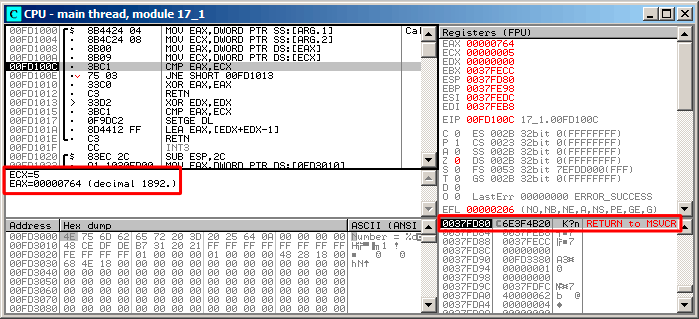
\includegraphics[scale=\FigScale]{patterns/18_pointers_to_functions/olly1.png}
\caption{\olly: first call of \comp}
\label{fig:qsort_olly1}
\end{figure}

\olly shows the compared values in the window under the code window, for convenience.
We can also see that the \ac{SP} points to \ac{RA}, where the \qsort function is (located in \TT{MSVCR100.DLL}).

\clearpage
By tracing (F8) until the \TT{RETN} instruction and pressing F8 one more time, we return to the \qsort function:

\begin{figure}[H]
\centering
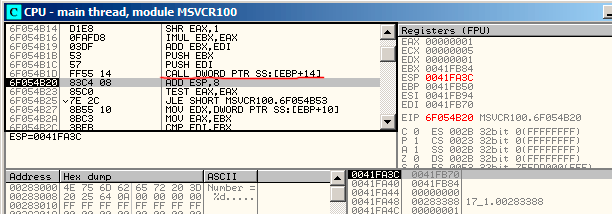
\includegraphics[scale=\FigScale]{patterns/18_pointers_to_functions/olly2.png}
\caption{\olly: the code in \qsort right after \comp call}
\label{fig:qsort_olly2}
\end{figure}

That was a call to the comparison function.

\clearpage
Here is also a screenshot of the moment of the second call of \comp{}---now values that have to be compared are different:

\begin{figure}[H]
\centering
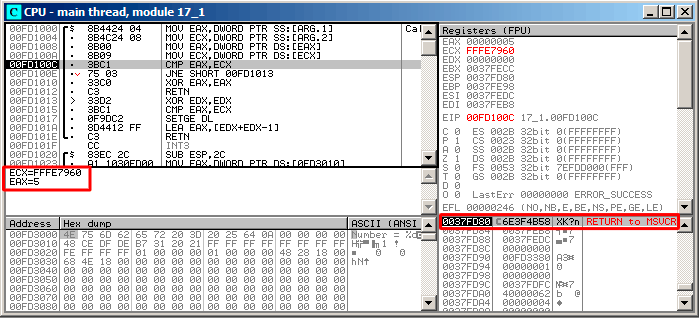
\includegraphics[scale=\FigScale]{patterns/18_pointers_to_functions/olly3.png}
\caption{\olly: second call of \comp}
\label{fig:qsort_olly3}
\end{figure}
